\documentclass[a4paper,11pt]{article}
\usepackage[T1]{fontenc}
\usepackage[utf8]{inputenc}
\usepackage{lmodern}
\usepackage[margin=2.4cm]{geometry}
\usepackage{amsmath,amssymb}
\usepackage{graphicx}
\usepackage{booktabs}
\usepackage{tabularx}
\usepackage{longtable}
\usepackage{array}
\usepackage{xcolor}
\usepackage{listings}
\usepackage{tikz}
\usetikzlibrary{arrows.meta,positioning,calc}
\usepackage{siunitx}
\usepackage{caption}
\usepackage[hidelinks]{hyperref}

\graphicspath{{figures/}}
\sisetup{group-separator={,},group-minimum-digits=4}
\setlength{\emergencystretch}{2em}

\definecolor{codebg}{HTML}{F6F5F2}
\definecolor{codekw}{HTML}{2A78D6}
\definecolor{codecm}{HTML}{6E6D68}
\definecolor{codestr}{HTML}{B4501F}
\lstset{
  language=Python, basicstyle=\ttfamily\footnotesize, backgroundcolor=\color{codebg},
  keywordstyle=\color{codekw}\bfseries, commentstyle=\color{codecm}\itshape,
  stringstyle=\color{codestr}, frame=none, columns=fullflexible, keepspaces=true,
  breaklines=true, showstringspaces=false, xleftmargin=0.6em, framexleftmargin=0.6em,
  aboveskip=0.8em, belowskip=0.8em, upquote=true
}
\usepackage{xurl}
\DeclareUrlCommand\code{\urlstyle{tt}}
\newcommand{\Qmli}{Q_{MLI}}
\newcommand{\mdot}{\dot m}

\title{PhlyGreen Technical Manual: Hydrogen Tank\\[4pt]
\large Theory, implementation and usage of the cryogenic liquid-hydrogen tank model}
\author{PhlyGreen development team\\Sapienza University of Rome}
\date{Code state: November 2026, branch \texttt{main}}

\begin{document}
\maketitle

\begin{abstract}
\noindent This manual documents the cryogenic liquid-hydrogen (LH$_2$) tank of PhlyGreen. The
tank stores the hydrogen of the two fuel-cell configurations, \code{'Hydrogen'} and
\code{'FuelCellBattery'}. We describe the sizing model, which finds the shape and the number of
tanks, the wall thicknesses and the insulation, and returns the empty tank mass. We then describe
the heat-leak model and the transient model, which follows the tank pressure and the stored mass
along the mission, with self-pressurization, venting at the maximum pressure and a heater at the
minimum pressure. We also describe the simpler gravimetric-index model, which PhlyGreen uses when
no tank is configured, and how both models enter the take-off-weight closure. For each part we
give the equations as implemented, with the code symbols. Every number in the manual comes from
running the code on the reference configurations of \code{trunk/examples/common.py}. The scripts
that produce the numbers and the figures are in \code{manuals/tank/scripts/}.
\end{abstract}

\tableofcontents
\newpage

%% ======================================================================================
\section{Scope and overview}\label{sec:scope}
%% ======================================================================================

A fuel-cell aircraft carries its hydrogen as a saturated liquid at about \SI{21}{K} and a little
above atmospheric pressure. The tank must hold this liquid, survive the internal pressure and
the external pressure on its vacuum jacket, and limit the heat that leaks in from the warm
surroundings. The heat boils part of the liquid, so the pressure rises. A valve vents gas when
the pressure reaches its maximum, and a heater adds heat when the fuel draw pulls the pressure
below its minimum.

PhlyGreen offers two models of the hydrogen storage:
\begin{itemize}
\item \textbf{Cryogenic tank} (\code{LH2_Tank}). It is used when the aircraft configuration
  carries a \code{TankConfig} and CoolProp is installed. It sizes the geometry and the walls, and
  returns the empty tank mass. Its transient method \code{time_step} follows the tank state
  along the mission.
\item \textbf{Gravimetric index}. It is used otherwise. The empty tank mass follows from a fixed
  ratio of stored hydrogen to hydrogen plus tank, \code{EnergyConfig.h2_gravimetric_index}.
\end{itemize}

The tank model is a sizing model. It returns a mass to the take-off-weight closure. The transient
model is a post-processing step: the vented hydrogen and the heater power it computes do not
feed back into the sizing. The fuel cell that consumes the hydrogen is the subject of the
companion manual \emph{PhlyGreen Technical Manual: Fuel Cell}, and the use of the liquid
hydrogen as a heat sink is the subject of \emph{PhlyGreen Technical Manual: Thermal Management}.
Section~\ref{sec:tms} states how the two connect to the tank.

\paragraph{Where the code lives.} Table~\ref{tab:files} lists the files. The tank is not built
by \code{PhlyGreen/factory.py:build_aircraft}. \code{Aircraft.__init__} sets
\code{aircraft.tank=None}. The fuel-cell closures reset it to \code{None} at the start
(\code{Weight._physics_tank_class}) and assign an \code{LH2_Tank} to \code{aircraft.tank} at
every evaluation of the take-off weight when the cryogenic tank is used. The tank reads its inputs from
\code{aircraft.TankInput}, the dictionary form of \code{config/sections.py:TankConfig}, and from
the parameter database \code{TANK_Database}.

\begin{table}[htbp]
\centering\small
\caption{Source files of the hydrogen tank (paths relative to \texttt{trunk/PhlyGreen/}).}
\label{tab:files}
\begin{tabularx}{\textwidth}{@{}lX@{}}
\toprule
File & Content \\
\midrule
\code{Systems/Tank/Tank.py} & \code{LH2_Tank} (sizing, \code{_calculate_structure}, \code{get_heat_leak}, \code{time_step}); \code{get_isa_atmosphere} \\
\code{Systems/Tank/TANK_Database.py} & \code{TANK_Database}: entry \code{'Cryogenic_Tank'} and its alias \code{'Svensson_Default'} \\
\code{Systems/Tank/__init__.py} & package exports; importing it without CoolProp raises \code{ImportError} \\
\code{Weight/Weight.py} & \code{Hydrogen}, \code{FuelCellBattery}, \code{_hydrogen_tank_mass}, \code{_physics_tank_class} \\
\code{Mission/Mission.py} & \code{track_tank}, \code{compute_tank_history} (tank state over the ground legs and the mission) \\
\code{postprocess.py} & \code{compute_tank_history} (calls the mission method), \code{plot_tank_state} \\
\code{config/sections.py} & \code{TankConfig}; \code{EnergyConfig.h2_gravimetric_index}, \code{h2_fuel_margin}, \code{contingency_fuel} \\
\code{results.py} & \code{tank_mass}, \code{hex_mass}, \code{empty_weight} \\
\code{config/aircraft_config.py} & \code{AircraftConfig.tank} $\to$ \code{TankInput} \\
\bottomrule
\end{tabularx}
\end{table}

\paragraph{Reference designs.} All numbers in this manual come from
\code{manuals/tank/scripts/compute_data.py}. It uses the configurations of
\code{trunk/examples/common.py}:
\begin{itemize}
\item \textbf{H2-GI}: \code{hydrogen_config()}, an ATR-like fuel-cell aircraft with
  \SI{4560}{kg} payload, a \SI{750}{nmi} mission and a \SI{220}{nmi} diversion, the
  \code{PEMFC_GoodPerformance} stack at a design cell voltage of \SI{0.5}{V}, a Class-I
  thermal-management system and the gravimetric-index tank with index 0.35. It is the reference
  design of the fuel-cell and thermal-management manuals.
\item \textbf{H2-T}: \code{hydrogen_config(tank=True)}, the same aircraft with the cryogenic
  tank, \code{TankConfig(max_diameter=2.4,number_of_tanks=1,tank_model='Svensson_Default')}.
\item \textbf{FCB-T}: \code{fuelcell_battery_config(tank=True)}, the fuel-cell + battery
  aircraft with a Class-I battery that supplies 15\,\% of the cruise power, and the same tank
  configuration.
\end{itemize}
The stand-alone studies of Section~\ref{sec:results} size an \code{LH2_Tank} directly, with
the same tank inputs, for the hydrogen mass that H2-T stores (\SI{461.0}{kg}). CoolProp
version 7.2.0 was used.

%% ======================================================================================
\section{Tank sizing model}\label{sec:sizing}
%% ======================================================================================

\code{LH2_Tank.__init__(capacity_kg,aircraft,allow_auto_split=True)} sizes the tank for a
total stored hydrogen mass $m_{H_2}$ (\code{capacity_kg}, stored as \code{m_tot_capacity}).
It reads three required keys of \code{TankInput}: \texttt{'Max Diameter'} $D_{max}$,
\texttt{'Number of Tanks'} $n$ (the starting number) and \texttt{'Tank Model'} (a key of
\code{TANK_Database}), and the optional \texttt{'Max Number of Tanks'} $n_{max}$. A missing
required key or a missing database parameter raises a \code{ValueError}. Without
\texttt{'Max Number of Tanks'}, $n_{max} = 4$ (\code{DEFAULT_MAX_NUMBER_OF_TANKS}); the
comment in \code{Tank.py} calls this cap an unsourced engineering assumption that stands for
the installation limit of a real aircraft. An explicit \code{None} removes the cap, and a
starting number above $n_{max}$ raises a \code{ValueError}. Figure~\ref{fig:section}
shows the construction.

\begin{figure}[htbp]
\centering
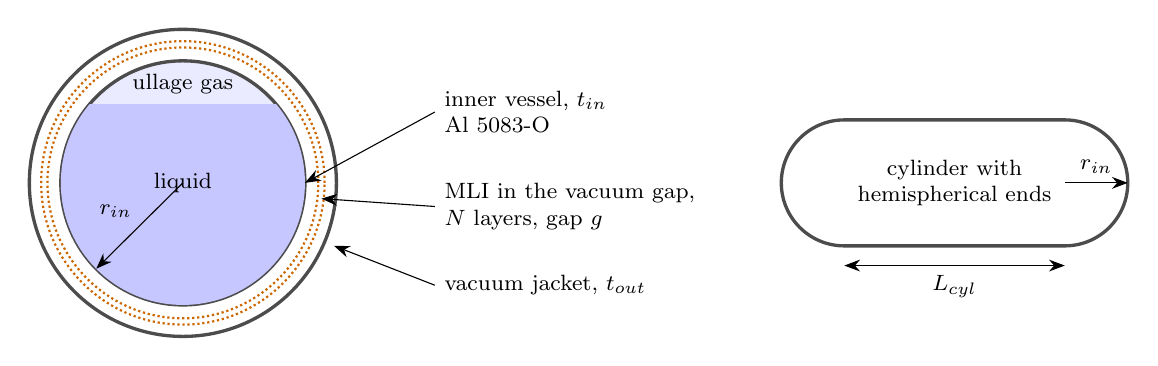
\begin{tikzpicture}[>={Stealth[length=2mm]}, font=\footnotesize]
  % sphere cross-section: inner wall, MLI gap, outer jacket
  \fill[blue!8] (0,0) circle (1.55);
  \draw[very thick, black!70] (0,0) circle (1.55);
  \draw[densely dotted, orange!80!black, thick] (0,0) circle (1.72);
  \draw[densely dotted, orange!80!black, thick] (0,0) circle (1.80);
  \draw[very thick, black!70] (0,0) circle (1.95);
  \fill[blue!20] (-1.45,-0.55) rectangle (1.45,-0.56);
  \begin{scope}
    \clip (0,0) circle (1.55);
    \fill[blue!22] (-1.6,-1.6) rectangle (1.6,1.0);
  \end{scope}
  \node at (0,0.0) {liquid};
  \node at (0,1.25) {ullage gas};
  \draw[->] (0,0) -- (-1.1,-1.09) node[midway, above left=-1pt] {$r_{in}$};
  \draw[<-] (1.55,0) -- (3.2,0.9) node[right, align=left] {inner vessel, $t_{in}$\\ Al 5083-O};
  \draw[<-] (1.76,-0.2) -- (3.2,-0.3) node[right, align=left] {MLI in the vacuum gap,\\ $N$ layers, gap $g$};
  \draw[<-] (1.92,-0.8) -- (3.2,-1.3) node[right, align=left] {vacuum jacket, $t_{out}$};
  % cylinder sketch
  \begin{scope}[xshift=9.8cm]
    \draw[very thick, black!70] (-1.4,-0.8) -- (1.4,-0.8) arc (-90:90:0.8) -- (-1.4,0.8) arc (90:270:0.8);
    \draw[<->] (-1.4,-1.05) -- (1.4,-1.05) node[midway, below] {$L_{cyl}$};
    \draw[->] (1.4,0) -- (2.2,0) node[midway, above] {$r_{in}$};
    \node[align=center] at (0,0) {cylinder with\\ hemispherical ends};
  \end{scope}
\end{tikzpicture}
\caption{Construction of one tank. Left: spherical tank (regime~1). Right: cylindrical tank with
hemispherical ends (regime~2), whose radius is fixed by the diameter limit. The drawing is not
to scale.}
\label{fig:section}
\end{figure}

\subsection{Database parameters}\label{sec:database}
Table~\ref{tab:database} lists the parameters of the only database entry,
\code{'Cryogenic_Tank'}, which \code{'Svensson_Default'} aliases. The header of
\code{TANK_Database.py} states that the data come from Svensson et al.~\cite{svensson}, and the
comments refer the insulation and the heat-leak constants to Table~4 of that paper. The
comment on \code{p_mli} states that the value was inferred by reverse engineering: the
``\SI{1}{mbar}'' of the paper is read as a typing error for \SI{1}{\micro bar}. The value
stored is $10^{-3}$\,Torr, which is \SI{1.33}{\micro bar}. Section~\ref{sec:leak} shows that
this parameter controls the heat leak. The Poisson ratio \code{nu_al} is not read.

\begin{table}[htbp]
\centering\small
\caption{Parameters of \texttt{TANK\_Database['Svensson\_Default']}.}\label{tab:database}
\begin{tabularx}{\textwidth}{@{}llrlX@{}}
\toprule
Key & Symbol & Value & Unit & Meaning \\
\midrule
\code{max_p_bar} & $P_{max}$ & 1.6 & bar & vent pressure \\
\code{min_p_bar} & $P_{min}$ & 1.2 & bar & minimum operating pressure (heater) \\
\code{sigma_y} & $\sigma_y$ & $228\times10^{6}$ & Pa & yield strength, Al 5083-O \\
\code{rho_al} & $\rho_{al}$ & 2660 & kg/m$^3$ & wall density \\
\code{E_al} & $E$ & $71\times10^{9}$ & Pa & Young's modulus \\
\code{nu_al} & $\nu$ & 0.33 & -- & Poisson ratio (not used) \\
\code{sf_inner} & $s_{in}$ & 2.0 & -- & safety factor on burst \\
\code{sf_outer} & $s_{out}$ & 2.5 & -- & safety factor on buckling \\
\code{ew} & $e_w$ & 0.80 & -- & weld efficiency \\
\code{buckling_knockdown} & $k_b$ & 0.36 & -- & knock-down factor for geometric imperfection \\
\code{accessory_mass_factor} & $f_{acc}$ & 1.35 & -- & structure-mass multiplier for accessories \\
\code{n_layers_mli} & $N$ & 9 & -- & number of MLI layers \\
\code{t_foam} & $t_{foam}$ & 0 & m & foam thickness (none in flight) \\
\code{rho_foam} & $\rho_{foam}$ & 35 & kg/m$^3$ & foam density \\
\code{insulation_gap} & $g$ & 0.03 & m & vacuum gap between the walls \\
\code{C1}, \code{C2} & $C_1$, $C_2$ & $4.43\times10^{-11}$, 3.91 & -- & solid conduction \\
\code{C3} & $C_3$ & $8.03\times10^{-10}$ & -- & radiation \\
\code{Cg}, \code{ng} & $C_g$, $n_g$ & $1.46\times10^{4}$, 0.53 & -- & gas conduction \\
\code{p_mli} & $p_{MLI}$ & $10^{-3}$ & Torr & residual gas pressure in the MLI \\
\code{Nt} & $N_t$ & 20 & layers/cm & layer density \\
\code{eps} & $\varepsilon$ & 0.03 & -- & layer emissivity \\
\bottomrule
\end{tabularx}
\end{table}

The constructor sets $P_{max}$ = \code{max_p_bar}$\times10^5$ and $P_{min} =
\max(\texttt{min\_p\_bar}, 1.2)\times10^5$\,Pa (\code{LH2_Tank.__init__}). A database entry
with a minimum pressure below \SI{1.2}{bar} is raised to \SI{1.2}{bar} with a
\code{RuntimeWarning}; the comment calls the floor an unsourced engineering assumption.

\subsection{Internal volume}\label{sec:volume}
The liquid density $\rho_l$ is the CoolProp density of saturated liquid para-hydrogen at
$P_{min}$. If CoolProp fails at this call the code uses \SI{70}{kg/m^3} and issues a
\code{RuntimeWarning}. Table~\ref{tab:props} gives the saturation properties that the model uses.
The internal volume of one tank is
\begin{equation}
  V = \frac{m_{H_2}/n}{\rho_l}\,(1 + u), \qquad u = 0.04,
  \label{eq:volume}
\end{equation}
with the ullage fraction $u$ = \code{ullage_frac} fixed in the code (an unsourced
engineering assumption). At $P_{min}$ the full tank
therefore holds liquid in 96.15\,\% of its volume.

\begin{table}[htbp]
\centering\small
\caption{Saturated para-hydrogen from CoolProp 7.2.0: temperature, liquid and vapour densities,
latent heat $\Delta h = h_g - h_l$, and $\rho^* = \rho_g/(\rho_l - \rho_g)$.}\label{tab:props}
\begin{tabular}{@{}rrrrrr@{}}
\toprule
$P$ [bar] & $T_{sat}$ [K] & $\rho_l$ [kg/m$^3$] & $\rho_g$ [kg/m$^3$] & $\Delta h$ [kJ/kg] & $\rho^*$ [--] \\
\midrule
1.2 & 20.86 & 70.15 & 1.560 & 443.2 & 0.0227 \\
1.6 & 21.92 & 68.85 & 2.030 & 436.5 & 0.0304 \\
2.0 & 22.80 & 67.69 & 2.497 & 429.4 & 0.0383 \\
3.0 & 24.57 & 65.16 & 3.670 & 410.6 & 0.0597 \\
\bottomrule
\end{tabular}
\end{table}

\subsection{Shape and number of tanks}\label{sec:shape}
The largest inner radius allowed is $R_{lim} = D_{max}/2 - 0.15$\,m. The clearance of
\SI{0.15}{m} is fixed in the code and has no source. The sphere of radius $R_{lim}$ has the volume
$V_{sph} = \tfrac43\pi R_{lim}^3$. The sizing loop runs as follows.
\begin{enumerate}
\item With the current number of tanks $n$, compute $V$ from~\eqref{eq:volume}.
\item If $V \le V_{sph}$, the tank is a sphere with $r_{in} = (3V/4\pi)^{1/3}$ and
  $L_{cyl} = 0$. The loop ends.
\item Otherwise the tank is a cylinder with hemispherical ends, $r_{in} = R_{lim}$ and
  $L_{cyl} = (V - V_{sph})/(\pi R_{lim}^2)$. If $L_{cyl} > 20\,r_{in}$ and $n < n_{max}$, $n$
  grows by one and the loop restarts. At $n = n_{max}$ the long cylinder is kept with a
  \code{RuntimeWarning}.
\item With \code{allow_auto_split=False}, or at $n = n_{max}$, the cylinder is kept. Otherwise
  the code also sizes the layout with $n+1$ tanks and compares the gravimetric
  indices~\eqref{eq:gi}. It keeps $n$ tanks if their index is at least as large; otherwise it
  moves to $n+1$ tanks and restarts the loop.
\end{enumerate}
The number of tanks can only grow from its input value, up to $n_{max}$. The aspect
limit $L_{cyl} \le 20\,r_{in}$ has no source in the code. The wetted inner area of one tank is
$A_{in} = 4\pi r_{in}^2 + 2\pi r_{in} L_{cyl}$ (\code{area_inner_tot}).

\subsection{Inner vessel}\label{sec:inner}
The inner vessel carries the internal pressure. The code designs it for $P_{d,in} =
2.2\,P_{max}$; the comment explains the factor as a 10\,\% valve overpressure times a factor of
2.0 for dynamic flight loads; the code calls the factor 2.2 an unsourced engineering
assumption. The comment refers to Eq.~3 of Svensson et
al.~\cite{svensson}. The thin-wall membrane thicknesses are
\begin{equation}
  t_{in,sph} = \max\!\left(\frac{P_{d,in}\, r_{in}\, s_{in}}{2\,\sigma_y\, e_w},\ t_{min}\right),
  \qquad
  t_{in,cyl} = \max\!\left(\frac{P_{d,in}\, r_{in}\, s_{in}}{\sigma_y\, e_w},\ t_{min}\right),
  \label{eq:tinner}
\end{equation}
with the minimum gauge $t_{min} = \SI{0.8}{mm}$ (\code{min_gauge}). The cylinder
thickness is used only for a cylindrical tank. The mass is
$m_{in} = \rho_{al}\,(4\pi r_{in}^2\, t_{in,sph} + 2\pi r_{in} L_{cyl}\, t_{in,cyl})$.

\subsection{Vacuum jacket}\label{sec:outer}
The outer wall carries the external atmospheric pressure on the vacuum gap. The code uses a
design pressure $P_{d,out} = 2 \times \SI{101325}{Pa}$ and the buckling formula that its comment
attributes to Eqs.~6 and~7 of Svensson et al.\ and to NASA SP-8007. The
jacket sits outside the inner wall and the vacuum gap, at the radius
$r_j = r_{in} + \max(t_{in,cyl}, t_{in,sph}) + g$, and this radius enters the formula:
\begin{equation}
  t_{out,sph} = \max\!\left(r_j\sqrt{\frac{P_{d,out}\, s_{out}^2}{k_b\, E}},\ t_{min}\right),
  \qquad
  t_{out,cyl} = \max\!\left(2.5\, t_{out,sph},\ t_{min}\right).
  \label{eq:touter}
\end{equation}
The factor 2.5 for the cylindrical jacket has no source in the code. The jacket mass is
$m_{out} = \rho_{al}\,[4\pi r_j^2\, t_{out,sph} + 2\pi r_j L_{cyl}\, t_{out,cyl}]$.

\subsection{Insulation, accessories and the empty mass}\label{sec:mass}
The insulation mass uses the inner area and an MLI areal density of
\SI{0.0272}{kg/m^2} per layer, which the comment attributes to Svensson et al.\:
\begin{equation}
  m_{ins} = A_{in}\,(t_{foam}\,\rho_{foam} + 0.0272\,N).
\end{equation}
The structure mass is multiplied by an accessory factor that covers supports, valves and
piping. For a cylinder the code adds a penalty that grows with the aspect ratio:
\begin{equation}
  f = f_{acc} + \begin{cases} 0 & \text{sphere}\\ 0.15 + 0.20\,L_{cyl}/r_{in} & \text{cylinder}\end{cases},
  \label{eq:accfactor}
\end{equation}
\begin{equation}
  m_{tank,1} = f\,(m_{in} + m_{out}) + m_{ins},
  \qquad
  m_{tank} = n\, m_{tank,1}.
  \label{eq:mass}
\end{equation}
The two penalty constants have no source in the code. The gravimetric index of the tank system is
\begin{equation}
  GI = \frac{m_{H_2}}{m_{H_2} + m_{tank}},
  \label{eq:gi}
\end{equation}
(\code{gravimetric_index}), where $m_{H_2}$ is the total stored hydrogen. The outer radius is
$r_{out} = r_j + t_{out,cyl}$ and $D_{out} = 2 r_{out}$. The constructor
raises a \code{ValueError} when $D_{out} > D_{max}$, that is, when the clearance of
\SI{0.15}{m} does not hold the walls and the gap. This does not happen in any case of this
manual.

\subsection{Why the index hardly depends on the tank size}\label{sec:scaling}
For a sphere above the minimum gauge, the inner thickness~\eqref{eq:tinner} is proportional
to $r_{in}$ and the jacket thickness~\eqref{eq:touter} to $r_j$. Neglecting the gap $g$, the
inner-wall thickness and the insulation, $r_j \approx r_{in}$, and both wall masses scale with
$r_{in}^3$, as the stored hydrogen does:
\begin{equation}
  \frac{m_{in}}{m_{H_2}/n} = \frac{3.3\,P_{max}\,s_{in}\,(1+u)\,\rho_{al}}{\sigma_y\,e_w\,\rho_l},
  \qquad
  \frac{m_{out}}{m_{H_2}/n} = 3\,s_{out}\sqrt{\frac{P_{d,out}}{k_b E}}\;\frac{(1+u)\,\rho_{al}}{\rho_l}.
  \label{eq:scaling}
\end{equation}
Neither ratio contains the tank size. With the gap and the inner wall, the jacket ratio is
multiplied by $(r_j/r_{in})^3$. A sphere has therefore almost the same index at any
capacity, and a split into more spheres costs little. The gap $g$ is the only length
scale; it makes small spheres slightly heavier. A cylinder pays the larger jacket factor and the
accessory penalty, so the automatic split replaces it by spheres whenever the diameter limit
allows and the cap $n_{max}$ is not reached (Section~\ref{sec:sens}). The vent pressure enters the inner-wall ratio linearly, and the
inner wall is the only mass that depends on it.

%% ======================================================================================
\section{Heat leak}\label{sec:leak}
%% ======================================================================================

\code{get_heat_leak(T_fluid,T_amb_external)} returns the heat that enters one tank through
the multi-layer insulation, with the modified Lockheed equation named in the database comments:
\begin{equation}
  \Qmli = A_{in}\left[
  \underbrace{\frac{C_1 N_t^{C_2}\,(T_h + T_c)(T_h - T_c)}{2\,(N+1)}}_{\text{solid conduction}}
  + \underbrace{\frac{C_3\,\varepsilon\,(T_h^{4.67} - T_c^{4.67})}{N}}_{\text{radiation}}
  + \underbrace{\frac{C_g\,p_{MLI}\,(T_h^{n_g} - T_c^{n_g})}{N}}_{\text{gas conduction}}
  \right].
  \label{eq:leak}
\end{equation}
The cold temperature $T_c$ is the saturation temperature at the current tank pressure. The hot
temperature $T_h$ is the ambient static temperature of \code{LH2_Tank._ambient_temperature}:
the ISA temperature of the package atmosphere (\code{PhlyGreen.Utilities.Atmosphere}),
constant above the tropopause at \SI{11000}{m}, plus the mission temperature offset
\code{mission.DISA}, which is zero for a stand-alone tank. The module function
\code{get_isa_atmosphere(altitude, DISA)} returns the same temperature. The flux is
applied to the inner area $A_{in}$. The outer wall is assumed to be at the ambient temperature, so
the fuselage and the cabin do not shield the tank.

With the database values the gas conduction term dominates. At sea level and $T_c$ at
\SI{1.2}{bar} the three terms are 0.022 (solid conduction), 0.82 (radiation) and 24.5\,W/m$^2$ (gas conduction). The heat leak therefore depends almost
linearly on $p_{MLI}$, which is the value inferred in the database comment
(Section~\ref{sec:database}). It also scales as $1/N$ (Section~\ref{sec:leakres}).

%% ======================================================================================
\section{Transient model}\label{sec:transient}
%% ======================================================================================

\code{time_step(dt,m_dot_req_total,altitude)} advances the state of the tanks by one time step
$\Delta t$. The state is the liquid-plus-vapour mass of one tank $m$ (\code{m_curr}) and the
pressure $P$ (\code{P_curr}). All tanks are identical and share the feed: one tank supplies
$\mdot_l = \mdot_{req}/n$. The model is homogeneous: the tank holds a saturated mixture with
bulk density $\rho = m/V$, and the liquid and the vapour are at the same temperature
$T_{sat}(P)$. The constructor starts a full tank at $P_{min}$.

\subsection{Properties}
At every step the code calls CoolProp at the current pressure for $T_{sat}$, the saturated
enthalpies $h_l$, $h_g$ and densities $\rho_l$, $\rho_g$, and forms $\Delta h = h_g - h_l$ and
$\rho^* = \rho_g/(\rho_l - \rho_g)$. It also forms the energy derivative
\begin{equation}
  \phi = \frac{1}{\rho\,(\partial u/\partial P)_\rho},
  \qquad
  \left(\frac{\partial u}{\partial P}\right)_\rho \approx
  \frac{u(P + \delta P, \rho) - u(P, \rho)}{\delta P},\quad \delta P = \SI{100}{Pa},
  \label{eq:phi}
\end{equation}
where $u$ is the specific internal energy of the mixture (\code{phi}). This
$\phi$ is not the supplied power ratio of the hybrid configurations. If any CoolProp call fails,
the step uses fixed values ($\phi = 0.5$, $T_{sat} = \SI{20}{K}$,
$\Delta h = \SI{445}{kJ/kg}$, $\rho^* = 0.05$) and issues a \code{RuntimeWarning}.

\subsection{Pressure equation}
The pressure rate is
\begin{equation}
  \frac{dP}{dt} = \frac{2\,\phi}{V}\left(1.3\,\Qmli - \Delta h\,\rho^*\,\mdot_l\right),
  \qquad
  P^{k+1} = P^k + \frac{dP}{dt}\,\Delta t,
  \label{eq:dpdt}
\end{equation}
an explicit Euler step. The heat raises the pressure. The liquid draw lowers it, because the
vapour must fill the volume the liquid leaves, and the evaporation that supplies this vapour
takes the latent heat $\Delta h$ per unit vapour mass. The code gives no source for the factor
1.3 on the heat leak or for the factor 2 in front of $\phi$. We read the factor 1.3 as an
allowance for heat paths other than the MLI (supports, piping); this is our interpretation, not a
statement of the code. The pressure stays constant when the draw per tank equals
\begin{equation}
  \mdot_{bal} = \frac{1.3\,\Qmli}{\Delta h\,\rho^*}.
  \label{eq:mbal}
\end{equation}
A smaller draw raises the pressure; a larger draw lowers it.

\subsection{Regulation: vent and heater}
The updated pressure $P^{k+1}$ is limited to $[P_{min}, P_{max}]$.
\begin{itemize}
\item \textbf{Heater.} If $P^{k+1} < P_{min}$, the pressure is held at $P_{min}$ and the heater
  supplies the power that closes the gap in one step,
  \begin{equation}
    Q_{heater} = \frac{(P_{min} - P^{k+1})\,V}{2\,\phi\,\Delta t} \ge 0.
  \end{equation}
\item \textbf{Vent.} If $P^{k+1} > P_{max}$, the pressure is held at $P_{max}$ and the valve
  vents the vapour flow
  \begin{equation}
    \mdot_g = \max\!\left(0,\ \frac{1.3\,\Qmli - \Delta h\,\rho^*\,\mdot_l}{\Delta h\,(1 + \rho^*)}\right).
    \label{eq:vent}
  \end{equation}
  This is the flow that makes the bracket of~\eqref{eq:dpdt} vanish when a vapour outflow
  term $-\Delta h(1+\rho^*)\mdot_g$ is added to it.
\item Otherwise $P = P^{k+1}$.
\end{itemize}
The properties of the step are those at the old pressure, also when the pressure is clamped.
The mass then decreases by $(\mdot_l + \mdot_g)\Delta t$ and cannot become negative. When $m$
falls below \SI{1}{g} the step records an empty tank and a zero feed.

\subsection{History}
Every step appends to \code{tank.history}, as totals over all tanks: \code{t} [s], \code{P}
[bar], \code{m_tot} [kg], \code{Vent} [kg/s], \code{Q_in} = $n\Qmli$ [W], \code{Q_heater} [W],
\code{Alt} [m], \code{m_vent_cum} [kg] and \code{Consumption} = $\mdot_{req}$ [kg/s]. Each
entry is stamped with the time of the previous entry plus $\Delta t$, the end of its step;
on an empty history the first step is stamped zero. \code{log_state(t, altitude)} appends the
current state at the time \code{t} without advancing it, with zero feed, vent and heater
power. \code{Mission.compute_tank_history} uses it to record the full tank at the start of
taxi-out, so the following steps are stamped from there.

\subsection{What the model does not contain}
The model has no thermal stratification, no separate liquid and vapour temperatures and no
wall heat capacity. The heat leak is quasi-steady. The vent and the heater act instantly and
exactly at the limits. There is no ortho--para conversion: the fluid is para-hydrogen
throughout. The feed leaves as liquid. The structural sizing does not see the transient, and the
vented mass and the heater energy do not enter the weight closure.

%% ======================================================================================
\section{The gravimetric-index model}\label{sec:gi}
%% ======================================================================================

\code{Weight._hydrogen_tank_mass(m_h2,LH2_Tank,grav_index)} returns zero for no hydrogen. If
an \code{LH2_Tank} class is available it builds the tank, stores it in \code{aircraft.tank} and
returns \code{mass_system_empty}. Otherwise it inverts~\eqref{eq:gi} with a fixed index,
\begin{equation}
  m_{tank} = m_{H_2}\left(\frac{1}{GI} - 1\right),
  \label{eq:gimodel}
\end{equation}
with $GI$ = \code{EnergyConfig.h2_gravimetric_index} (key \texttt{'H2 Gravimetric Index'},
default 0.35 in \code{Weight.Hydrogen} and \code{Weight.FuelCellBattery}).
\code{Weight._physics_tank_class} returns the class when \code{aircraft.TankInput} is set and
the import of \code{LH2_Tank} from \code{PhlyGreen.Systems.Tank} succeeds. When a
\code{TankConfig} is given but the import fails (no CoolProp), it issues a
\code{RuntimeWarning} and the design uses~\eqref{eq:gimodel}. It first resets
\code{aircraft.tank} to \code{None}, so in that case \code{aircraft.tank} is \code{None}.

The gravimetric-index model has no geometry, no pressure and no transient. It does not depend
on the diameter limit or on the vent pressure. Section~\ref{sec:resgi} compares it with the
cryogenic tank.

%% ======================================================================================
\section{Coupling with the aircraft sizing}\label{sec:coupling}
%% ======================================================================================

\subsection{Stored hydrogen}\label{sec:load}
Both fuel-cell closures, \code{Weight.Hydrogen} and \code{Weight.FuelCellBattery}, compute the
hydrogen load from the hydrogen chemical energy $E_{H_2}$ that the mission returns. This energy
includes the flown profile (mission, diversion and loiter) and the ground segments (taxi-out,
take-off run and taxi-in). The fuel-cell manual describes how the mission computes it. The
closure adds the margin $\mu$ = \code{EnergyConfig.h2_fuel_margin} (default 0.05) for unusable
and residual hydrogen and the feed system:
\begin{equation}
  W_{H_2} = \frac{E_{H_2}}{e_f}\,(1 + \mu),
  \qquad
  W_{res} = \begin{cases} \texttt{contingency\_fuel} & \text{if given}\\ 0.05\,W_{H_2} & \text{otherwise}\end{cases},
  \qquad
  m_{H_2} = W_{H_2} + W_{res},
  \label{eq:load}
\end{equation}
where $e_f$ = \code{EnergyConfig.Ef} is the hydrogen higher heating value. The tank is sized for
the load plus the reserve, $m_{H_2}$ (\code{Weight.Hydrogen} and \code{Weight.FuelCellBattery}).

\subsection{Take-off-weight closure}
At every trial take-off weight the closure builds a tank through
\code{_hydrogen_tank_mass} and adds its empty mass $W_{tank}$ to the balance
\begin{equation}
  W_{structure} + W_{FC} + [W_{bat}] + W_{H_2} + W_{tank} + W_{TMS} + W_{payload} + W_{crew} + W_{res} - W_{TO} = 0,
\end{equation}
where $W_{bat}$ appears in the fuel-cell + battery closure only. The root is found by
\code{Weight._solve_wto}. The tank built at the last trial is the one left in
\code{aircraft.tank}; for the reference designs its capacity equals the converged
$m_{H_2}$ to numerical precision. \code{aircraft.results()} reports the empty tank mass as
\code{tank_mass} and the heat-exchanger mass as \code{hex_mass}, and both are part of
\code{empty_weight}, so that \code{empty_weight} + \code{WPayload} + \code{Wf} +
\code{final_reserve} = \code{WTO}. A lighter tank lowers the take-off weight, which lowers the
structure, the fuel cell and the hydrogen in turn.

\subsection{Tank state along the mission}\label{sec:track}
The transient model runs after the design, in one of two ways.
\begin{enumerate}
\item \code{aircraft.mission.track_tank=True}, followed by
  \code{aircraft.mission.EvaluateMission(aircraft.weight.WTO)}. For the \code{'Hydrogen'} and
  \code{'FuelCellBattery'} configurations, \code{EvaluateMission} then calls
  \code{Mission.compute_tank_history} after the flight; without a cryogenic tank it warns.
\item \code{postprocess.compute_tank_history(aircraft)}, which calls the same mission method
  on the stored solution and does not re-fly the mission.
\end{enumerate}
\code{Mission.compute_tank_history} resets the tank to full (its sized capacity) at $P_{min}$
and logs this state at the start of taxi-out. Time follows the profile clock, on which the
climb starts at zero, so taxi-out and the take-off run have negative times. The walk has
three parts:
\begin{enumerate}
\item taxi-out and the take-off run, at the constant hydrogen flows of the ground segments
  (\code{Mission._ground_segments}), at the take-off altitude, in steps of at most
  \SI{10}{s};
\item the flown profile: for each accepted step $[t_{k-1}, t_k]$ of the mission integrator it
  takes the hydrogen chemical-energy increment $\Delta E$ (the first ODE state), sets
  $\mdot_{req} = \Delta E / (e_f\,\Delta t)$ and the altitude at the mid-point, and calls
  \code{time_step}; the integrator steps are at most \SI{60}{s} long (\code{max_step=60.0});
\item taxi-in, after landing, as in the first part.
\end{enumerate}
The tank feeds all the hydrogen that the sizing counts as burnt, ground legs included. At the
end of the history it holds the margin $\mu$ and the reserve, less the vented mass. On H2-T and
FCB-T the two ways give identical histories.

\subsection{Relation with the fuel cell and the thermal-management system}\label{sec:tms}
The tank does not change the fuel cell or its hydrogen consumption. The Class-II
thermal-management system uses the liquid hydrogen as its first heat sink. It assumes that the
hydrogen leaves the tank as saturated liquid at a fixed supply pressure,
\code{TMSConfig.h2_supply_pressure}, with default \SI{1.6}{bar}, equal to the default
$P_{max}$. It does not read the tank pressure or the tank history.
%% ======================================================================================
\section{Results on the reference designs}\label{sec:results}
%% ======================================================================================

\subsection{The sized tank and the aircraft}\label{sec:resref}
Table~\ref{tab:designs} compares the three designs. On H2-T the tank holds \SI{461.0}{kg}
of hydrogen. The automatic split replaces the single cylinder of the input by two spheres of
\SI{0.934}{m} inner radius and \SI{1.946}{m} outer diameter, inside the \SI{2.4}{m} limit.
The empty tank system weighs \SI{720.6}{kg}, which gives a gravimetric index of 0.390.
This is higher than the index 0.35 of H2-GI, so the cryogenic tank is \SI{156.3}{kg} lighter and the
take-off mass falls by \SI{509}{kg} (2.4\,\%). The take-off mass falls about 3.3 times as much as the
tank mass, because the structure, the fuel cell and the hydrogen shrink with it.

\begin{table}[htbp]
\centering\small
\caption{Reference designs. Masses in kg. The stored hydrogen is $W_{H_2} + W_{res}$ and the
system index is the stored hydrogen over stored hydrogen plus tank. The empty weight is
\texttt{results().empty\_weight}, which contains the tank and the TMS.}\label{tab:designs}
\begin{tabular}{@{}lrrr@{}}
\toprule
 & H2-GI & H2-T & FCB-T \\
\midrule
Take-off mass $W_{TO}$ & 21634 & 21125 & 38638 \\
Structure & 11886 & 11623 & 20502 \\
Fuel-cell system & 2400 & 2343 & 4286 \\
Battery & 0 & 0 & 5137 \\
TMS & 940 & 918 & 1678 \\
Hydrogen load $W_{H_2}$ & 449.7 & 439.1 & 735.4 \\
Reserve $W_{res}$ & 22.5 & 22.0 & 36.8 \\
Stored hydrogen & 472.2 & 461.0 & 772.2 \\
Empty tank $W_{tank}$ & 876.9 & 720.6 & 1203.3 \\
System index [--] & 0.350 & 0.390 & 0.391 \\
Empty weight & 16602 & 16104 & 33306 \\
\midrule
Tank model & index 0.35 & 2 spheres & 3 spheres \\
Inner radius / outer diameter [m] & -- & 0.934 / 1.946 & 0.969 / 2.017 \\
Design run time [s] & 25 & 26 & 27 \\
\bottomrule
\end{tabular}
\end{table}

Table~\ref{tab:breakdown} breaks down one H2-T tank. The vacuum jacket is the largest item: its
buckling thickness of \SI{6.80}{mm} is 3.8 times the pressure-wall thickness of \SI{1.80}{mm}. The
accessory factor adds a quarter of the tank mass. The nine MLI layers weigh less than
\SI{1}{\%} of it. The inner-wall and jacket masses per kilogram of hydrogen in one tank are
0.228 and 0.921. These are the two ratios of~\eqref{eq:scaling}, 0.228 and 0.833, with the
jacket ratio multiplied by $(r_j/r_{in})^3 = 1.106$.

\begin{table}[htbp]
\centering\small
\caption{Mass breakdown of one H2-T tank (two identical spheres).}\label{tab:breakdown}
\begin{tabular}{@{}lrrl@{}}
\toprule
Item & Mass [kg] & Share & Notes \\
\midrule
Inner vessel $m_{in}$ & 52.6 & 14.6\,\% & $t_{in}$ = 1.80\,mm \\
Vacuum jacket $m_{out}$ & 212.3 & 58.9\,\% & $t_{out}$ = 6.80\,mm \\
Accessories $(f-1)(m_{in}+m_{out})$ & 92.7 & 25.7\,\% & $f$ = 1.35 \\
Insulation $m_{ins}$ & 2.7 & 0.7\,\% & 9 MLI layers \\
\midrule
One tank $m_{tank,1}$ & 360.3 & 100\,\% & holds 230.5\,kg \\
\bottomrule
\end{tabular}
\end{table}

\subsection{Tank state over the mission}\label{sec:reshist}
Figure~\ref{fig:history} shows the H2-T tank from the start of taxi-out to the end of taxi-in,
obtained with \code{track_tank}. Taxi-out and the take-off run last \SI{822}{s}, so the
history starts at $t = -\SI{822}{s}$. The run of \code{EvaluateMission} with the tracking
takes \SI{3.9}{s}; \code{compute_tank_history} takes \SI{2.1}{s} and returns the same history.

\begin{figure}[htbp]
\centering
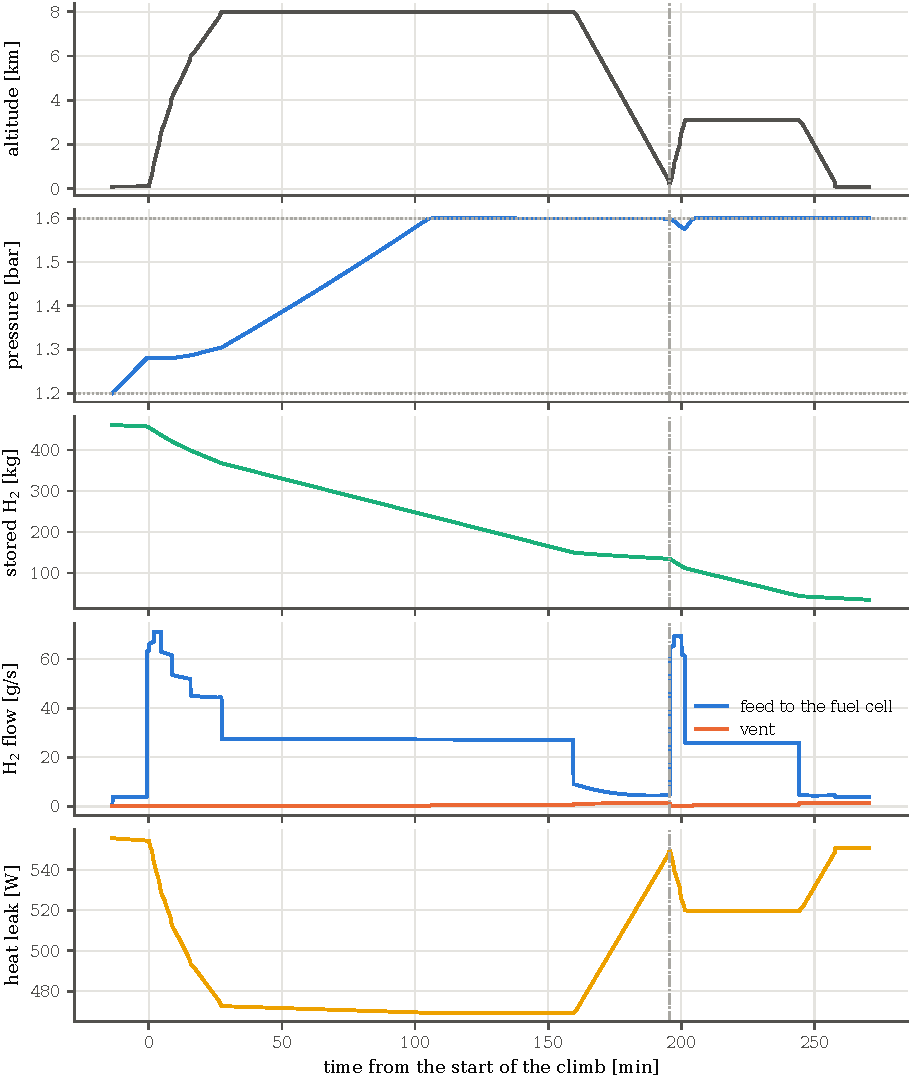
\includegraphics[width=\textwidth]{mission_history.pdf}
\caption{H2-T tank over taxi-out, take-off run, mission, diversion and taxi-in
(\texttt{track\_tank}); time from the start of the climb. From top: altitude, pressure with
the limits $P_{min}$ and $P_{max}$ (dotted), stored hydrogen of both tanks, hydrogen feed to
the fuel cell and vent flow, and heat leak. Dash-dotted line: end of the nominal mission.}
\label{fig:history}
\end{figure}

During taxi-out the feed is \SI{3.9}{g/s}, far below the balance draw~\eqref{eq:mbal}, and
the pressure rises; at the start of the climb it is \SI{1.281}{bar}. The take-off run draws
\SI{63.4}{g/s}. The largest feed, \SI{71.2}{g/s} in the climb, stays just below the balance
draw of both tanks at sea level and $P_{min}$, \SI{71.8}{g/s}, so the pressure keeps rising
slowly. In cruise the feed is less than half of that, so the heat leak raises the pressure at
a nearly constant rate. The pressure reaches $P_{max}$ \SI{106}{min} after the start of the
climb, during the cruise, and the valve vents from then on. The short dip at the start of the
diversion, down to \SI{1.576}{bar}, is the diversion climb. Its feed is close to that of the
mission climb, but at $P_{max}$ the product $\Delta h\,\rho^*$ is 32\,\% larger than at
$P_{min}$ (Table~\ref{tab:props}), so the balance draw is lower and the draw pulls the
pressure down. The heater is never used. From taxi-out to taxi-in the tank feeds
\SI{418.2}{kg} to the fuel cell, \SI{5.7}{kg} of it before the climb, and vents
\SI{8.72}{kg}. The fed mass equals the burnt hydrogen of the sizing, ground legs included. The
tank ends with \SI{34.1}{kg}: the margin $\mu$ (\SI{20.9}{kg}) and the reserve
(\SI{22.0}{kg}), less the vented mass. The heat leak varies between \SI{469}{W} at cruise
altitude and \SI{556}{W} at sea level; it follows the ambient temperature and, weakly, the
saturation temperature.

On FCB-T the three spheres hold \SI{772.2}{kg}. Its largest feed, \SI{130.2}{g/s} in the
climb, exceeds its balance draw at sea level and $P_{min}$, \SI{115.9}{g/s}, so the climb
lowers the pressure. The ground legs have raised it to \SI{1.277}{bar} before the climb, and
the lowest pressure in the climb is \SI{1.269}{bar}; the heater is not used. The valve opens
\SI{108}{min} after the start of the climb and vents \SI{13.5}{kg}. The \code{track_tank}
history and \code{compute_tank_history} agree exactly.

The vented mass is not part of the sizing. On H2-T it is 20\,\% of the margin $\mu$ and
the reserve together. Whether the margin should cover it is a design choice that the code leaves to
the user.

\subsection{Sizing sensitivities}\label{sec:sens}
\paragraph{Capacity and splitting.} Figure~\ref{fig:capacity} sizes stand-alone tanks with
$D_{max} = \SI{2.4}{m}$ and a starting number of one tank. Up to \SI{300}{kg} one sphere fits.
Above it a single cylinder grows long and its index falls quickly, from 0.356 at
\SI{350}{kg} to 0.198 at \SI{1500}{kg}, because of the jacket factor 2.5 and the accessory
penalty. With the automatic split the model adds spheres instead, and up to \SI{1200}{kg}
(four spheres) the index stays between 0.369 and 0.392, as~\eqref{eq:scaling} predicts. At
\SI{1500}{kg} the cap of four tanks stops the split: the model keeps four cylinders, with an
index of 0.345. Without the cap it chooses five spheres, with an index of 0.392. The automatic
split keeps a cylinder only at the cap in the sweeps of this manual.

\begin{figure}[htbp]
\centering
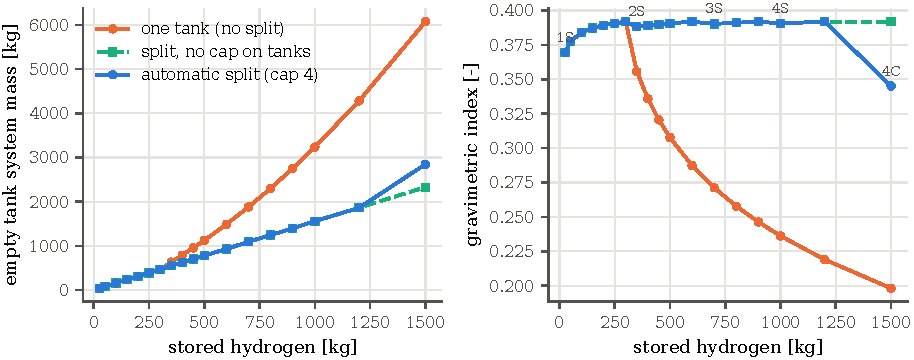
\includegraphics[width=\textwidth]{capacity_sweep.pdf}
\caption{Stand-alone tanks versus stored hydrogen ($D_{max} = \SI{2.4}{m}$, one starting tank).
Left: empty tank system mass. Right: gravimetric index; labels give the number of tanks and
the shape (S: sphere, C: cylinder) chosen by the automatic split with the default cap of four
tanks. Dashed: the split without a cap.}
\label{fig:capacity}
\end{figure}

\paragraph{Diameter limit.} Figure~\ref{fig:diameter} (left) sizes the H2-T hydrogen mass for
several diameter limits. With the split, a smaller diameter means more spheres, from one
sphere at \SI{2.8}{m} and above to four spheres at \SI{1.8}{m}, and the index changes only from
0.394 to 0.385. Below \SI{1.8}{m} four spheres cannot hold the hydrogen and the cap of four
tanks stops the split: the model keeps four cylinders, with an index of 0.303 at \SI{1.6}{m}
and 0.248 at \SI{1.4}{m}. Without the cap the split would choose six and ten spheres, with
indices of 0.382 and 0.377. Without the split a single cylinder at \SI{1.4}{m} has an index
of 0.126. The right panel repeats the sweep with full aircraft designs. From \SI{2.0}{m} to
\SI{3.2}{m} the take-off mass changes by \SI{75}{kg}. At \SI{1.6}{m} the four cylinders weigh
\SI{1177}{kg} and the take-off mass rises to \SI{22610}{kg}, \SI{1484}{kg} above the
\SI{2.4}{m} design. The diameter limit is a weak design driver as long as the cap on the
number of tanks is not reached.

\begin{figure}[htbp]
\centering
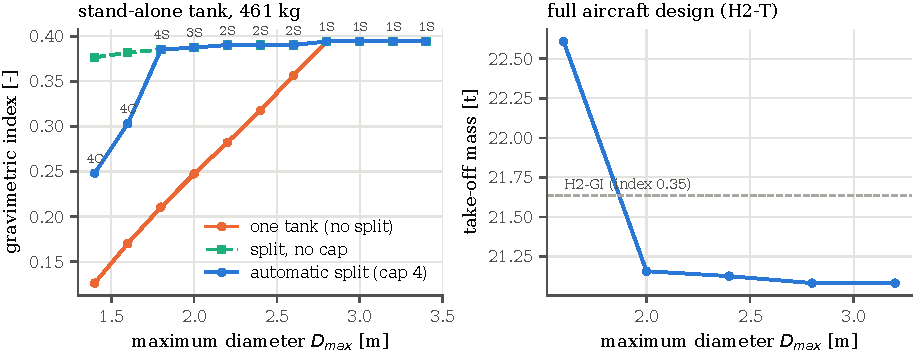
\includegraphics[width=\textwidth]{diameter_sweep.pdf}
\caption{Effect of the diameter limit. Left: stand-alone tank for the H2-T hydrogen mass;
labels give the number of tanks and the shape (S: sphere, C: cylinder) with the default cap
of four tanks; dashed: the split without a cap. Right: take-off mass of full H2-T designs;
dashed line: H2-GI.}
\label{fig:diameter}
\end{figure}

\paragraph{Starting number of tanks.} With the split the starting number matters only when it
is larger than the number the split would choose, because the split never removes a tank.
For the H2-T hydrogen mass, one or two starting tanks give the same two spheres
(\SI{720.6}{kg}); three and four give \SI{729.1}{kg} and \SI{736.0}{kg} of tank mass.

\paragraph{Vent pressure.} Table~\ref{tab:pmax} raises $P_{max}$ through database entries added at run time.
Only the inner wall grows, linearly with $P_{max}$, as~\eqref{eq:scaling} states; the liquid
volume is unchanged because the density is taken at $P_{min}$. On full designs the take-off
mass grows by \SI{303}{kg} at \SI{2.5}{bar} and by \SI{649}{kg} at \SI{3.5}{bar}.

\begin{table}[htbp]
\centering\small
\caption{Effect of the vent pressure $P_{max}$ on the stand-alone tank for the H2-T hydrogen
mass, and on full H2-T designs.}\label{tab:pmax}
\begin{tabular}{@{}rrrrrr@{}}
\toprule
$P_{max}$ [bar] & $t_{in,sph}$ [mm] & $m_{tank}$ [kg] & $GI$ [--] & $W_{TO}$ [kg] & $W_{tank}$ in design [kg] \\
\midrule
1.6 & 1.80 & 720.6 & 0.390 & 21125 & 720.6 \\
2.0 & 2.25 & 756.9 & 0.379 & -- & -- \\
2.5 & 2.82 & 802.3 & 0.365 & 21428 & 813.6 \\
3.0 & 3.38 & 847.7 & 0.352 & -- & -- \\
3.5 & 3.94 & 893.2 & 0.340 & 21775 & 920.0 \\
4.0 & 4.51 & 938.6 & 0.329 & -- & -- \\
5.0 & 5.64 & 1029.4 & 0.309 & -- & -- \\
\bottomrule
\end{tabular}
\end{table}

\paragraph{Gravimetric-index model.}\label{sec:resgi} Table~\ref{tab:gisweep} sweeps the index
of the simple model on H2-GI. The cryogenic tank of H2-T, with its index of 0.390, closes at
\SI{21125}{kg}, between the simple model at 0.35 and at 0.40, and \SI{106}{kg} heavier than
the latter. Each step of 0.05 in the index changes the
take-off mass by \SIrange{0.46}{1.34}{t} in this range.

\begin{table}[htbp]
\centering\small
\caption{Full designs with the gravimetric-index model (H2-GI with a changed index).}\label{tab:gisweep}
\begin{tabular}{@{}rrrr@{}}
\toprule
$GI$ [--] & $W_{TO}$ [kg] & $W_{tank}$ [kg] & stored H$_2$ [kg] \\
\midrule
0.25 & 23851 & 1561.6 & 520.5 \\
0.30 & 22509 & 1146.2 & 491.2 \\
0.35 & 21634 & 876.9 & 472.2 \\
0.40 & 21019 & 688.1 & 458.7 \\
0.45 & 20563 & 548.5 & 448.8 \\
\bottomrule
\end{tabular}
\end{table}

\subsection{Heat leak and insulation}\label{sec:leakres}
Figure~\ref{fig:leak} (left) shows the three terms of~\eqref{eq:leak} versus the ambient
temperature. The gas conduction term is 96.7\,\% of the flux at sea level. The total heat
of the two H2-T tanks falls from \SI{557}{W} at sea level to \SI{443}{W} at \SI{11000}{m}. The right
panel varies the number of layers through database entries added at run time. The flux follows $1/N$ closely:
\SI{1002}{W} for 5 layers, \SI{557}{W} for 9 and \SI{125}{W} for 40 (both tanks, sea level). From 9
to 40 layers the insulation mass grows from \SI{5.4}{kg} to \SI{23.9}{kg}, a small change of the
tank mass.

\begin{figure}[htbp]
\centering
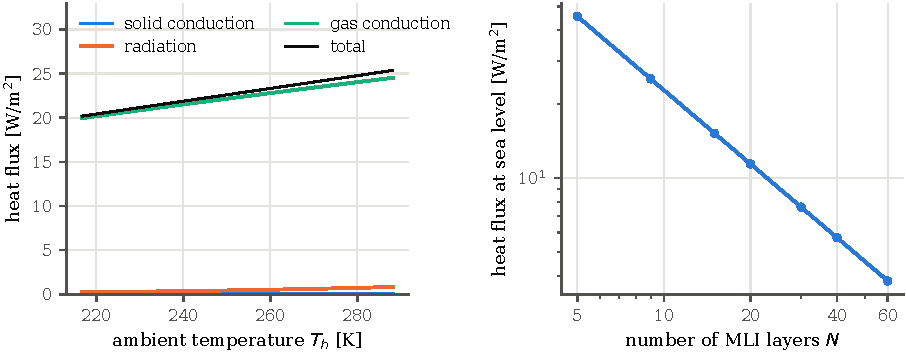
\includegraphics[width=\textwidth]{heat_leak.pdf}
\caption{Heat flux through the MLI of the H2-T tank, cold side at $T_{sat}(\SI{1.2}{bar})$.
Left: the three terms of~\eqref{eq:leak} versus the ambient temperature (\SI{9}{layers}). Right:
total flux at sea level versus the number of layers.}
\label{fig:leak}
\end{figure}

\subsection{Parked tank and time step}\label{sec:parked}
A full H2-T tank with no draw reaches $P_{max}$ after \SI{57}{min} at sea level and after
\SI{67}{min} at \SI{8000}{m} (Figure~\ref{fig:parked}). It then vents \SI{1.60}{g/s} at sea level. Over
\SI{24}{h} it loses 28.7\,\% of its hydrogen at sea level and 24.2\,\% at \SI{8000}{m}. These
values reflect the flight insulation of the database, nine MLI layers and no foam; the model has
no ground insulation or ground cooling.

\begin{figure}[htbp]
\centering
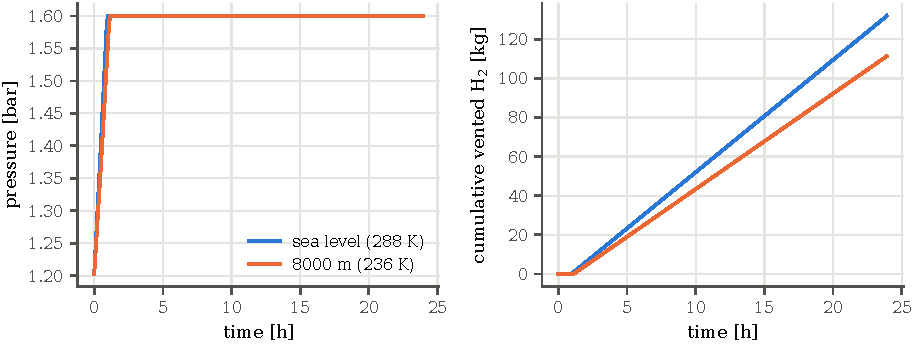
\includegraphics[width=\textwidth]{parked.pdf}
\caption{Full H2-T tank with no draw, $\Delta t = \SI{30}{s}$. Left: pressure. Right: cumulative
vented hydrogen.}
\label{fig:parked}
\end{figure}

The explicit step~\eqref{eq:dpdt} converges well at the step sizes the mission uses. For the
parked tank at sea level, the time to $P_{max}$ is \SI{3423}{s} with $\Delta t = \SI{1}{s}$,
\SI{3420}{s} with \SI{60}{s} and \SI{3360}{s} with \SI{120}{s}; the mass vented in \SI{6}{h} changes
by less than \SI{0.4}{\%}. Replaying the H2-T feed with each step split into
five sub-steps changes the vented mass from \SI{8.716}{kg} to \SI{8.714}{kg}.

\paragraph{Heavy draw.} A draw of \SI{0.5}{kg/s} from the full H2-T tank at sea level, seven
times the largest mission feed, holds the pressure at $P_{min}$ with a heater power of up to
\SI{4317}{W}.

\subsection{Mission feed on tank variants}\label{sec:replay}
The transient does not feed back into the design, so the H2-T feed, ground legs included, can
be replayed on stand-alone tank variants (Figure~\ref{fig:replay}, Table~\ref{tab:replay}). The
replay of the reference tank reproduces the tracked history exactly. A higher vent pressure
delays the vent and reduces the vented mass: at \SI{3.0}{bar} the tank reaches $P_{max}$ only
during taxi-in and vents \SI{0.20}{kg}, at the price of \SI{127.1}{kg} of tank mass. More
insulation removes the vent, but the slower pressure rise then lets the climb feed pull the
pressure down to $P_{min}$, and the heater has to work. This
trade between heat leak and heater power is a direct consequence of~\eqref{eq:mbal}.

\begin{figure}[htbp]
\centering
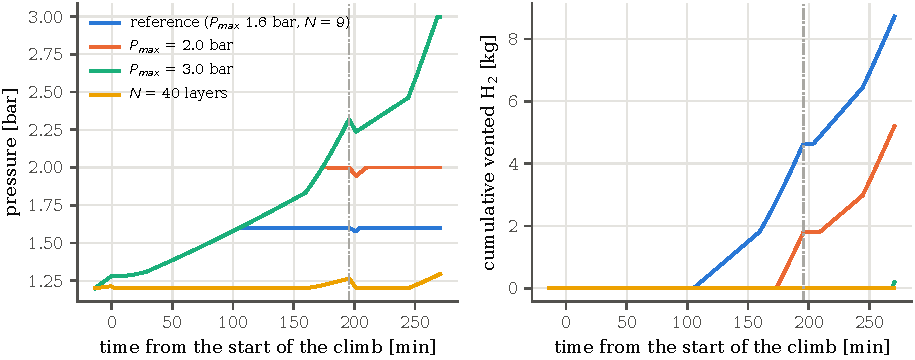
\includegraphics[width=\textwidth]{replay.pdf}
\caption{H2-T feed (taxi-out to taxi-in) replayed on tank variants; time from the start of the
climb. Left: pressure. Right: cumulative vented hydrogen. Dash-dotted line: end of the nominal
mission.}
\label{fig:replay}
\end{figure}

\begin{table}[htbp]
\centering\small
\caption{H2-T feed replayed on tank variants (both tanks). Reference: $P_{max} = \SI{1.6}{bar}$,
$N = 9$. The vent time is counted from the start of the climb.}\label{tab:replay}
\begin{tabular}{@{}lrrrrr@{}}
\toprule
Variant & $m_{tank}$ [kg] & $P_{peak}$ [bar] & vent from [min] & vented [kg] & $Q_{heater,max}$ [W] \\
\midrule
reference & 720.6 & 1.600 & 106 & 8.72 & 0 \\
$P_{max}$ = 2.0 bar & 756.9 & 2.000 & 174 & 5.21 & 0 \\
$P_{max}$ = 3.0 bar & 847.7 & 3.000 & 268.5 & 0.20 & 0 \\
$N$ = 20 layers & 727.2 & 1.570 & -- & 0.00 & 238 \\
$N$ = 40 layers & 739.1 & 1.295 & -- & 0.00 & 561 \\
reference, 5 sub-steps & 720.6 & 1.600 & 105 & 8.71 & 0 \\
\bottomrule
\end{tabular}
\end{table}

%% ======================================================================================
\section{Usage}\label{sec:usage}
%% ======================================================================================

The snippets run from \code{trunk/} with the package installed in the \code{phlygreen}
environment, which has CoolProp.

\subsection{Typed configuration}
A \code{TankConfig} attached to the \code{AircraftConfig} of a fuel-cell aircraft selects the
cryogenic tank:
\begin{lstlisting}
import sys; sys.path.insert(0, 'examples')
import PhlyGreen as pg
from PhlyGreen.config import TankConfig
from common import hydrogen_config

config = hydrogen_config()             # gravimetric-index tank (index 0.35)
config.tank = TankConfig(max_diameter=2.4, number_of_tanks=1,
                         tank_model='Svensson_Default')
# equivalent: config = hydrogen_config(tank=True)

aircraft = pg.build_aircraft()
aircraft.configure(config)             # about 30 s

w, tank = aircraft.weight, aircraft.tank
print(w.WH2_Fuel, w.final_reserve, w.WTank)          # load, reserve, empty tank [kg]
r = aircraft.results()
print(r.tank_mass, r.hex_mass, r.empty_weight)      # tank and TMS are in the empty weight
print(tank.shape, tank.n_tanks, tank.r_inner, tank.D_outer, tank.gravimetric_index)
print(tank.mass_inner, tank.mass_outer, tank.mass_insulation)   # per tank [kg]
\end{lstlisting}
\code{fuelcell_battery_config(tank=True)} does the same for the fuel-cell + battery aircraft.
\code{aircraft.results()} reports the hydrogen as \code{Wf} and \code{final_reserve}, the empty
tank as \code{tank_mass} and the heat exchangers as \code{hex_mass}; the geometry is in
\code{aircraft.tank}. \code{TankConfig(max_number_of_tanks=...)} changes the cap of four tanks
on the automatic split. Without a \code{TankConfig}, the index is set with
\code{config.energy.h2_gravimetric_index}.

\subsection{Legacy dictionaries}
The same inputs go into the \code{TankInput} dictionary:
\begin{lstlisting}
aircraft.DesignAircraft(AerodynamicsInput, ConstraintsInput, MissionInput, EnergyInput,
                        MissionStages, DiversionStages,
                        TankInput={'Max Diameter': 2.4, 'Number of Tanks': 1,
                                   'Tank Model': 'Svensson_Default',
                                   'Max Number of Tanks': 4})
\end{lstlisting}

\subsection{Tank state over the mission}
\begin{lstlisting}
# Re-fly the mission with the tracking on (both fuel-cell configurations) ...
aircraft.mission.track_tank = True
aircraft.mission.EvaluateMission(aircraft.weight.WTO)
h = aircraft.tank.history            # t, P, m_tot, Vent, Q_in, Q_heater, Alt, m_vent_cum, Consumption

# ... or walk the stored mission solution without re-flying it:
from PhlyGreen import postprocess
h = postprocess.compute_tank_history(aircraft)
postprocess.plot_tank_state(aircraft)   # pressure, stored mass, vent flow, heater power
print(max(h['P']), h['m_vent_cum'][-1], max(h['Q_heater']))
\end{lstlisting}

\subsection{A stand-alone tank}
The constructor only reads \code{TankInput} from the aircraft object, so a small stand-in is
enough. This is how the studies of Section~\ref{sec:results} were made:
\begin{lstlisting}
from PhlyGreen.Systems.Tank import LH2_Tank, TANK_Database

class TankOnlyAircraft:
    TankInput = {'Max Diameter': 2.4, 'Number of Tanks': 1, 'Tank Model': 'Svensson_Default'}

tank = LH2_Tank(capacity_kg=461.0, aircraft=TankOnlyAircraft())   # default cap: 4 tanks
for _ in range(120):                        # one hour parked at sea level
    tank.time_step(dt=30.0, m_dot_req_total=0.0, altitude=0.0)

params = dict(TANK_Database['Svensson_Default'])   # a variant, in memory only
params['max_p_bar'] = 3.0
TANK_Database['my_tank'] = params                   # then TankConfig(tank_model='my_tank')
\end{lstlisting}

\subsection{Examples}
\begin{itemize}
\item \code{examples/22_hydrogen_tank.py} sizes H2-T, prints the tank, re-flies the mission with
  \code{track_tank} and plots pressure, stored mass, feed, vent flow and heat flows.
\item \code{examples/20_hydrogen_fuel_cell.py} and \code{23_fuelcell_battery_hybrid.py} use the
  gravimetric-index tank.
\item \code{docs/user-guide/hydrogen.md}, Section~6, is the user guide of the tank;
  \code{docs/api/tank.md} renders the docstrings of \code{Tank.py}.
\end{itemize}

\subsection{Pitfalls}
\begin{itemize}
\item \textbf{Fallback without CoolProp.} Without CoolProp a \code{TankConfig} is ignored, with a
  \code{RuntimeWarning}, and the gravimetric index is used; \code{aircraft.tank} is then
  \code{None}.
\item \textbf{Starting number of tanks.} \code{number_of_tanks} is a lower bound, not the result.
  Read \code{tank.n_tanks}. Pass \code{allow_auto_split=False} to the constructor to keep the
  cylinder; the weight closure always uses the default \code{True}.
\item \textbf{Cap on the number of tanks.} The split stops at \code{max_number_of_tanks}
  (default 4, unsourced). Above it the model keeps cylinders, which are much heavier
  (Section~\ref{sec:sens}). Check for the \code{RuntimeWarning} of a long cylinder.
\item \textbf{Diameter limit.} \code{max_diameter} limits the inner radius to
  $D_{max}/2 - \SI{0.15}{m}$, and the sized outer diameter must stay below it.
  \code{TankConfig.fuselage_diameter} is not read by the model.
\item \textbf{History time.} The tank history starts full at the start of taxi-out, at a
  negative time on the profile clock. The final mass is the margin and the reserve less the
  vented hydrogen.
\item \textbf{Variants.} Database variants added at run time live only in the running process.
\end{itemize}

%% ======================================================================================
\section{Verification and limitations}\label{sec:verification}
%% ======================================================================================

\subsection{Tests}
The following tests cover the tank. We ran \code{test_hydrogen_tank.py} and
\code{test_ground_segments.py} on the code described here; all 39 tests passed (24 in the first file, four of them slow, and 15 in the second).
\begin{itemize}
\item \code{tests/regression/test_hydrogen_tank.py} (skipped without CoolProp): a sized tank
  has a positive mass, an index between 0 and 1, a valid shape and $P_{min} < P_{max}$; more
  hydrogen needs a heavier tank; with no draw the pressure rises, reaches $P_{max}$ exactly
  and never exceeds it, and gas is vented; a draw depletes the mass monotonically; a heavy
  draw engages the heater and the pressure never falls below $P_{min}$. The slow tests size a
  hydrogen aircraft with a tank, check \code{WTank} against \code{mass_system_empty}, track the
  mission and check the pressure limits, the consumption and the ground legs in the history,
  and fill the history of a fuel-cell + battery aircraft through \code{track_tank}. Further
  tests cover the warnings without CoolProp or without a physics tank, the CoolProp fallbacks,
  the ambient temperature with \code{DISA}, the jacket radius in the buckling formula, the
  floor on $P_{min}$, the outer-diameter check, the cap on the number of tanks and its
  validation in \code{TankConfig}, and \code{log_state}.
\item \code{tests/regression/test_ground_segments.py}: the gravimetric-index tank holds the load
  plus the reserve, $W_{tank} = (W_{H_2} + W_{res})(1/GI - 1)$; the margin $\mu$ is an
  explicit input.
\item \code{tests/regression/test_hydrogen.py}, \code{test_fuelcell_battery.py} and
  \code{test_tms_design.py} check that $W_{tank}$ is positive and closes the weight balance with
  the gravimetric-index model.
\end{itemize}
The computations of Section~\ref{sec:results} add four consistency checks. First, the tracked
history and \code{compute_tank_history} agree exactly on H2-T and FCB-T, and so does the replay
of the recorded feed. Second, the H2-T history closes its mass balance: the start mass minus
the fed and the vented hydrogen equals the end mass, and the fed hydrogen equals the burnt
hydrogen of the sizing, ground legs included. Third, the inner-wall and jacket ratios of
Table~\ref{tab:breakdown} match~\eqref{eq:scaling}. Fourth, the three terms of~\eqref{eq:leak},
summed by the script, equal \code{get_heat_leak}.

\subsection{Limitations}
\begin{itemize}
\item \textbf{Sources.} The database cites Svensson et al.\ for the materials, the insulation and
  the heat-leak constants. The following constants of \code{Tank.py} have no source in the code:
  the clearance of \SI{0.15}{m}, the ullage fraction 0.04, the aspect limit of 20, the cap of
  four tanks, the floor of \SI{1.2}{bar} on $P_{min}$, the minimum gauge, the factor 2.2 on the
  inner design pressure, the jacket factor 2.5 for cylinders, the cylinder accessory penalty
  $0.15 + 0.20\,L_{cyl}/r_{in}$, and the factors 1.3 and 2 of~\eqref{eq:dpdt}. The residual gas
  pressure of the MLI, which sets the heat leak, is an inferred value.
\item \textbf{Geometry.} Only spheres and cylinders with hemispherical ends are modelled, with
  no integral or conformal tanks. The number of tanks is capped at an unsourced default of four.
  There is no check of the installation against the fuselage, and the tank does not change the
  fuselage or the structure model.
\item \textbf{Structure.} Thin-wall membrane and buckling formulas with safety factors; no
  fatigue, no thermal stress, no supports.
\item \textbf{Heat leak.} The outer wall is at the ambient static temperature (ISA plus the
  mission offset \code{DISA}). There is no fuselage shielding and no ground insulation.
\item \textbf{Transient.} Homogeneous saturated mixture, explicit Euler steps, no
  stratification and no wall heat capacity; the vent and the heater are ideal. The vented
  hydrogen and the heater energy do not enter the sizing. The ground legs are flown at the
  take-off altitude with constant flows.
\item \textbf{Properties.} CoolProp failures fall back to fixed values with a warning, at
  sizing (liquid density) and at every time step.
\end{itemize}

%% ======================================================================================
\appendix
\section{Input reference}\label{app:inputs}
%% ======================================================================================

Table~\ref{tab:inputs} lists the inputs that act on the hydrogen storage. ``req.'' means that
the code reads the key without a default. The database parameters are in
Table~\ref{tab:database}.

\begin{table}[htbp]
\centering\scriptsize
\caption{Hydrogen-storage inputs: typed field, legacy key, default, unit and meaning.}\label{tab:inputs}
\setlength{\tabcolsep}{3pt}
\begin{tabularx}{\textwidth}{@{}>{\raggedright\arraybackslash}p{3.3cm}>{\raggedright\arraybackslash}p{3.3cm}lp{0.8cm}>{\raggedright\arraybackslash}X@{}}
\toprule
Field & Legacy key & Default & Unit & Meaning \\
\midrule
\multicolumn{5}{@{}l}{\emph{\code{TankConfig} (\texttt{TankInput})}}\\
\code{max_diameter} & \texttt{Max Diameter} & req. & m & $D_{max}$; inner radius $\le D_{max}/2 - 0.15$, $D_{out} \le D_{max}$ \\
\code{number_of_tanks} & \texttt{Number of Tanks} & 1 & -- & starting number of tanks, $\ge 1$ \\
\code{max_number_of_tanks} & \texttt{Max Number of Tanks} & 4 & -- & cap $n_{max}$ on the split (unsourced); \code{None} in a dictionary removes it \\
\code{tank_model} & \texttt{Tank Model} & \code{'Svensson_Default'} & -- & key of \code{TANK_Database} \\
\code{fuselage_diameter} & \texttt{Fuselage Diameter} & \code{None} & m & not read by the model \\
\midrule
\multicolumn{5}{@{}l}{\emph{\code{EnergyConfig} (\texttt{EnergyInput})}}\\
\code{h2_gravimetric_index} & \texttt{H2 Gravimetric Index} & 0.35 & -- & $GI$ of~\eqref{eq:gimodel}, used without a cryogenic tank \\
\code{h2_fuel_margin} & \texttt{H2 Fuel Margin} & 0.05 & -- & margin $\mu$ on the hydrogen load \\
\code{contingency_fuel} & \texttt{Contingency Fuel} & 5\,\% of $W_{H_2}$ & kg & reserve $W_{res}$, stored in the tank \\
\code{Ef} & \texttt{Ef} & req. & J/kg & $e_f$, the hydrogen HHV (141.87\,MJ/kg in \code{common.py}) \\
\midrule
\multicolumn{5}{@{}l}{\emph{Attributes and arguments}}\\
\code{Mission.track_tank} & -- & \code{False} & -- & run \code{compute_tank_history} in \code{EvaluateMission} \\
\code{LH2_Tank(allow_auto_split=...)} & -- & \code{True} & -- & compare $n$ and $n+1$ tanks \\
\bottomrule
\end{tabularx}
\end{table}

\code{TankConfig.__post_init__} checks that \code{max_diameter} is positive when given, that
\code{number_of_tanks} is at least one, and that \code{max_number_of_tanks}, when given, is at
least one and not below \code{number_of_tanks}.

\section{Reproducing the figures}

\begin{lstlisting}[language=bash]
cd trunk
python ../manuals/tank/scripts/make_figures.py --recompute     # phlygreen environment
cd ../manuals/tank && latexmk -pdf -interaction=nonstopmode -outdir=build tank_manual.tex
\end{lstlisting}
\code{compute_data.py} runs the designs and the tank studies and writes
\code{data/tank_data.json} (about 9 minutes). \code{plots.py} draws the figures from it into
\code{figures/} in a few seconds. Without \code{--recompute} the driver reuses the JSON file.

%% ======================================================================================
\begin{thebibliography}{9}\small
\bibitem{svensson} C.~Svensson et al., \emph{Modelling hydrogen fuel cell aircraft in SUAVE},
ICAS 2024. Source of \code{TANK_Database.py}.
\end{thebibliography}


\end{document}
